% Vietnamese translation for OI Public Library
% Source-PDF: IOI中国国家候选队论文/2009/金斌/slide.pdf
\documentclass[11pt]{article}
\usepackage{tikz}
\usetikzlibrary{arrows.meta,calc}
\usepackage{oipl-vn}
\renewcommand{\figurename}{Hình}

\newcommand{\Oh}{\mathcal{O}}
\newcommand{\abs}[1]{\left|#1\right|}
\newcommand{\floor}[1]{\left\lfloor #1\right\rfloor}
\newcommand{\vect}[1]{\overrightarrow{#1}}

\title{Ứng dụng của thuật toán Euclid}
\author{Kim Bân\\Trường Trung học Cao cấp Thường Châu, Giang Tô}
\date{Tháng 1 năm 2009}

\begin{document}
\maketitle

\origtitle{Applications of the Euclidean Algorithm}
\sourcepath{IOI-China-Candidate-Team-Papers/2009/Jin-Bin/slide.pdf}

\section{Tổng quan}

Bài trình bày xoay quanh thuật toán Euclid và một số cách dùng không chỉ dừng
ở bài toán ước chung lớn nhất. Mạch nội dung của slide gồm:
\begin{enumerate}
  \item thuật toán Euclid, tức phép chia lấy dư liên tiếp;
  \item thuật toán Euclid mở rộng và phương trình đồng dư tuyến tính;
  \item các thuật toán Euclid theo nghĩa rộng hơn;
  \item liên phân số và phương trình Pell;
  \item ví dụ WifiPlanet trong TopCoder SRM 410 Hard.
\end{enumerate}

Trong phần trình bày này, trọng tâm được đặt vào ba mảng: thuật toán Euclid
cơ bản, thuật toán Euclid hai chiều, và ví dụ WifiPlanet.

\section{Thuật toán Euclid}

\subsection{Chia lấy dư liên tiếp}

Vì đây là thuật toán cơ bản nhất của lý thuyết số, ta có thể viết trực tiếp
mã giả:

\begin{verbatim}
Algorithm Euclidean Algorithm
Input: x >= 0 and y >= 0
Output: the greatest common divisor of x and y
 1: while y != 0 do
 2:     t <- x mod y
 3:     x <- y
 4:     y <- t
 5: end while
 6: return x
\end{verbatim}

Ý tưởng cốt lõi là liên tục thay cặp số đang xét bằng một cặp nhỏ hơn nhưng
không đổi ước chung lớn nhất. Nếu $x=qy+r$, thì mọi ước chung của $x,y$ cũng
là ước của $r=x\bmod y$, và mọi ước chung của $y,r$ cũng là ước của $x$. Vì
vậy
\[
  \gcd(x,y)=\gcd(y,x\bmod y).
\]

\subsection{Phân tích độ phức tạp}

Với hai số bất kỳ $a,b$ thỏa mãn $a>b>0$, xét hiệu quả của thao tác
\[
  a\gets a\bmod b. \tag{1}
\]

Nếu $b\le a/2$, thì $a\bmod b<b\le a/2$. Nếu $b>a/2$, thì
\[
  a\bmod b\le a-b<a-a/2=a/2.
\]
Như vậy mỗi thao tác dạng (1) đều làm $a$ giảm ít nhất một nửa, nên số bước
của thuật toán là $\Oh(\log n)$ nếu bỏ qua chi phí của phép chia trên số lớn.

\section{Các thuật toán Euclid khác thường}

Dễ hình dung rằng bất kỳ hai ``số'' nào có phép lấy modulo và phù hợp với một
thứ tự bộ phận đều có thể áp dụng tư tưởng Euclid; đa thức là một ví dụ quen
thuộc. Ta còn có thể đi xa hơn: phóng đại phép lấy modulo thành biến đổi sơ
cấp của ma trận, hoặc thành thao tác trên vector hai chiều.

\section{Thuật toán Euclid hai chiều}

\subsection{Đề bài}

\paragraph{Bài toán.}
Maloyaroslavets Summer Camp 2008 đưa ra bài toán sau: cho hai vector $a,b$,
tìm các số nguyên $x,y$ không đồng thời bằng $0$ sao cho
\[
  \abs{ax+by}
\]
nhỏ nhất.

Để tiện thảo luận, ta quy ước $a\cdot b\ge 0$, tức $a$ và $b$ cùng hướng, và
\[
  \abs a\le \abs b.
\]
Nếu dùng $a$ và $b$ làm hai trục tọa độ xiên, các điểm có dạng $ax+by$ chính
là lưới sinh bởi hai vector đó. Bài toán trở thành tìm điểm lưới khác gốc
$O$ có khoảng cách tới $O$ nhỏ nhất.

\begin{figure}[ht]
\centering
\begin{tikzpicture}[
  >=Stealth,
  every node/.style={font=\small},
  dot/.style={circle,fill=black,inner sep=1.6pt}
]
\coordinate (O) at (0,0);
\coordinate (A) at (1.15,0);
\coordinate (B) at (.52,.82);
\foreach \i in {-1,0,...,4} {
  \foreach \j in {-1,0,...,3} {
    \node[dot] at ($\i*(A)+\j*(B)$) {};
  }
}
\draw[->,thick] (O) -- ($(O)+4.6*(A)$) node[right] {trục \(a\)};
\draw[->,thick] (O) -- ($(O)+3.5*(B)$) node[above] {trục \(b\)};
\node[below left] at (O) {$O$};
\draw[->,blue!65!black,thick] (O) -- (A) node[midway,below] {\(a\)};
\draw[->,red!70!black,thick] (O) -- (B) node[midway,left] {\(b\)};
\end{tikzpicture}
\caption{Lưới sinh bởi hai vector \(a,b\); bài toán là tìm điểm lưới khác \(O\) gần \(O\) nhất.}
\end{figure}

Khi góc giữa hai vector càng nhỏ, lưới càng dẹt và bài toán càng khó nhìn ra
ngay. Một trường hợp đặc biệt rất gợi ý là khi $a$ và $b$ cộng tuyến: đáp án
khi đó chính là $\gcd(\abs a,\abs b)$. Nếu góc giữa $a$ và $b$ nhỏ đến mức có
thể xem như gần cộng tuyến, trực giác vẫn dẫn ta về ước chung lớn nhất. Vì
thế lời giải tổng quát phải chứa thuật toán Euclid thông thường như một
trường hợp con.

\subsection{Hai kết luận cơ bản}

\paragraph{Kết luận 1.}
Nếu góc giữa $a,b$ lớn hơn $\pi/3$, thì đáp án cần tìm là
\[
  \min(\abs a,\abs b).
\]

\paragraph{Chứng minh.}
Đặt $p=\abs a$, $q=\abs b$, và giả sử $p\le q$. Gọi $\alpha$ là góc giữa hai
vector. Khi đó
\[
\begin{aligned}
  \abs{ax+by}
    &=\sqrt{(px)^2+(qy)^2-2pxqy\cos\alpha}\\
    &\ge \sqrt{\abs{px}^2+\abs{qy}^2-2\abs{px}\abs{qy}\cos\alpha}\\
    &\ge \sqrt{\abs{px}^2+\abs{qy}^2-\abs{px}\abs{qy}}\\
    &\ge \sqrt{(\abs{px}-\abs{qy})^2+\abs{px}\abs{qy}}.
\end{aligned}
\]
Nếu $x=0$ thì $y\ne0$, do đó
$(\abs{px}-\abs{qy})^2=\abs{qy}^2\ge q^2\ge p^2$. Nếu $y=0$ thì $x\ne0$,
do đó $(\abs{px}-\abs{qy})^2=\abs{px}^2\ge p^2$. Trong trường hợp cả hai đều
khác $0$, ta có $\abs{px}\abs{qy}\ge pq\ge p^2$. Vậy mọi tổ hợp khác $0$ đều
có độ dài ít nhất $p$, còn chọn $(x,y)=(1,0)$ đạt đúng $p$.

\paragraph{Kết luận 2.}
Đáp án ứng với cặp $(a,b)$ giống đáp án ứng với cặp $(a,b+ka)$, trong đó $k$
là số nguyên.

\paragraph{Chứng minh.}
Giả sử $\abs{ax+by}$ là giá trị cần tìm. Khi đó
\[
  \abs{a(x-ky)+(b+ka)y}
\]
cũng bằng giá trị ấy. Nghiệm $(x,y)$ tương ứng với nghiệm $(x-ky,y)$, và nếu
$(x,y)\ne(0,0)$ thì $(x-ky,y)\ne(0,0)$. Chiều ngược lại chứng minh tương tự,
vì phép biến đổi có thể đảo bằng cách dùng $-k$.

Hai kết luận này cho ta cả điều kiện dừng lẫn dạng biến đổi. Điều cần làm là
liên tục dùng kết luận 2 để làm tăng góc giữa hai vector, cho đến khi góc vượt
quá $\pi/3$.

\subsection{Cách chọn phép biến đổi}

Ta nhắc lại quy ước $\abs a\le\abs b$. Trong hình học của slide, đặt
\[
  \vect{OA}=a,\qquad \vect{OB}=b.
\]
Gọi $E$ là hình chiếu của $B$ lên đường thẳng $OA$. Chọn số nguyên $k$ sao cho
$C$ và $D$ là hai điểm liên tiếp trên tia $OA$ bao quanh $E$:
\[
  \vect{OC}=k\vect{OA},\qquad
  \vect{OD}=(k+1)\vect{OA}.
\]

\begin{figure}[ht]
\centering
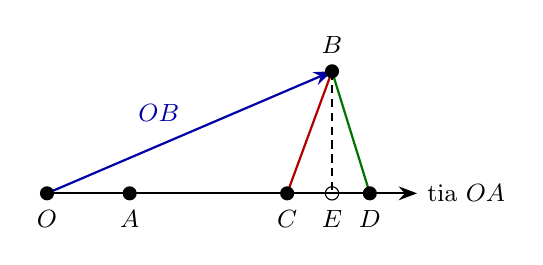
\begin{tikzpicture}[
  >=Stealth,
  every node/.style={font=\small},
  dot/.style={circle,fill=black,inner sep=1.8pt},
  open/.style={circle,draw,inner sep=1.7pt}
]
\coordinate (O) at (0,0);
\coordinate (A) at (1.05,0);
\coordinate (C) at (3.05,0);
\coordinate (E) at (3.62,0);
\coordinate (D) at (4.1,0);
\coordinate (B) at (3.62,1.55);
\draw[->,thick] (O) -- (4.7,0) node[right] {tia \(OA\)};
\draw[->,blue!65!black,thick] (O) -- (B) node[midway,above left] {\(OB\)};
\draw[densely dashed] (B) -- (E);
\draw[thick,red!70!black] (C) -- (B);
\draw[thick,green!45!black] (D) -- (B);
\foreach \p/\lab in {O/O,A/A,C/C,D/D} {
  \node[dot,label=below:{\(\lab\)}] at (\p) {};
}
\node[open,label=below:{\(E\)}] at (E) {};
\node[dot,label=above:{\(B\)}] at (B) {};
\end{tikzpicture}
\caption{Chọn \(C=kA\) và \(D=(k+1)A\) là hai bội liên tiếp của \(A\) bao quanh hình chiếu \(E\) của \(B\); sau đó thay \((OA,OB)\) bằng \((CB,OA)\) hoặc \((DB,OA)\).}
\end{figure}

Nếu $\abs{OA}>\abs{OE}$, ta có thể chứng minh
\[
  \angle OAB>\angle AOB,
\]
chẳng hạn bằng cách lấy điểm đối xứng $A'$ của $A$ qua $E$. Trường hợp còn
lại, ta so sánh $\abs{CE}$ và $\abs{DE}$:
\begin{itemize}
  \item nếu $\abs{CE}<\abs{DE}$, thay cặp $(OA,OB)$ bằng $(CB,OA)$;
  \item nếu không, thay cặp $(OA,OB)$ bằng $(DB,OA)$.
\end{itemize}

Phép thay này vẫn thuộc dạng $(a,b)\mapsto(a,b+ka)$ kết hợp với đổi thứ tự hai
vector. Một kết luận hình học được dùng trong slide là
\[
  \max(\angle BCE,\angle BDE)>\angle AOB.
\]
Thật vậy, có thể chứng minh trực tiếp
\[
  \angle DCB=\angle AOB+\angle CBO>\angle AOB.
\]
Do đó biến đổi trên luôn làm góc giữa hai vector tăng lên.

Vì vậy thuật toán dựa trên Euclid đã thành hình: mỗi bước dùng một bài toán
bậc hai đơn giản để tính giá trị $k$, thực hiện biến đổi tương ứng, rồi lặp
cho đến khi góc vượt quá $\pi/3$. Tác giả không đưa ra chứng minh chặt cho độ
phức tạp; theo thực nghiệm, thuật toán thường kết thúc sau vài bước và có vẻ
ở cấp $\Oh(\log C)$.

\section{WifiPlanet}

\subsection{Đề bài}

\paragraph{Bài toán.}
TopCoder SRM 410 Hard, WifiPlanet, tác giả đề là bmerry: trên mặt phẳng lưới
nguyên có một đa giác đơn, các đỉnh có tọa độ hữu tỉ. Hỏi bên trong đa giác có
bao nhiêu điểm lưới. Đề bài đảm bảo không có điểm lưới nào nằm trên biên.

\subsection{Phân tích bằng phân hoạch hình thang}

Một phản xạ tự nhiên là thử tam giác phân đa giác, nhưng với bài toán đếm
điểm lưới, phân hoạch hình thang phù hợp hơn:
\[
  \text{tam giác phân?}\qquad \text{phân hoạch hình thang!}
\]

Sau khi cắt theo các đường thẳng đứng qua các đỉnh, bài toán quy về việc đếm
số điểm lưới dưới một đoạn thẳng. Với đoạn có độ dốc $k$ và tung độ đầu $b$,
số điểm cần cộng có dạng
\[
  \sum_{i=0}^{n-1}\floor{b+ki}.
\]
Khi viết $b$ và $k$ dưới dạng hữu tỉ, biểu thức chuẩn của bài toán trở thành
\[
  \sum_{i=0}^{n-1}\floor{\frac{a+di}{m}}. \tag{2}
\]

\begin{figure}[ht]
\centering
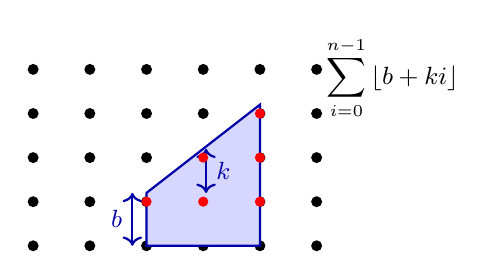
\begin{tikzpicture}[
  x=.72cm,y=.56cm,
  every node/.style={font=\small},
  dot/.style={circle,fill=black,inner sep=1.4pt}
]
\foreach \x in {0,...,5} {
  \foreach \y in {0,...,4} {
    \node[dot] at (\x,\y) {};
  }
}
\fill[blue!16] (2,0) -- (4,0) -- (4,3.2) -- (2,1.2) -- cycle;
\draw[blue!65!black,thick] (2,0) -- (4,0) -- (4,3.2) -- (2,1.2) -- cycle;
\draw[blue!65!black,thick,<->] (1.75,0) -- node[left] {\(b\)} (1.75,1.2);
\draw[blue!65!black,densely dashed] (2,1.2) -- (3,2.2);
\draw[blue!65!black,thick,<->] (3.05,1.2) -- node[right] {\(k\)} (3.05,2.2);
\foreach \p in {(2,1),(3,1),(3,2),(4,1),(4,2),(4,3)} {
  \node[circle,fill=red,inner sep=1.3pt] at \p {};
}
\node[anchor=west] at (5.0,3.8) {\(\displaystyle\sum_{i=0}^{n-1}\left\lfloor b+ki\right\rfloor\)};
\end{tikzpicture}
\caption{Phân hoạch hình thang của \textit{WifiPlanet}: đếm điểm lưới dưới đoạn thẳng dẫn tới tổng các phần nguyên.}
\end{figure}

\subsection{Thuật toán Euclid cho tổng phần nguyên}

Xét
\[
  S(a,d,m,n)=\sum_{i=0}^{n-1}\floor{\frac{a+di}{m}}.
\]
Ta đặt các quy ước:
\begin{itemize}
  \item $0\le a<m$; nếu không, có thể đưa $\floor{a/m}$ ra ngoài tổng.
  \item $0<d<m$; bằng cách tách phần nguyên của $d/m$ tương tự, có thể đưa bài
  toán về trường hợp này.
\end{itemize}
Tương đương theo tham số thực là $0\le b<1$ và $0<k<1$.

Ý nghĩa hình học của (2) là: từ các điểm
\[
  (i,a+di),\qquad i=0,1,\ldots,n-1,
\]
kẻ các tia thẳng đứng xuống dưới. Khi chia trục tung thành các mức
$0,m,2m,\ldots$, tổng (2) chính là số giao điểm giữa các tia đó và những
đường ngang này.

Đặt
\[
  l=\floor{\frac{a+dn}{m}}.
\]
Khi đó có $l$ đường thẳng ngang cần xét. Gọi
\[
  \mathit{topY}=a+dn,
\]
và với đường ngang thứ $k$ đặt $\mathit{nowY}=mk$. Số điểm giao tương ứng với
đường ngang đó là
\[
  \floor{\frac{\mathit{topY}-\mathit{nowY}}{d}}.
\]
Nhìn theo hướng này, ta đã hoán đổi hai cạnh của hình chữ nhật/hình thang:
thay vì cộng theo từng tia dọc, ta cộng theo từng đường ngang.

Do
\[
  \mathit{topY}-mk=(a+dn)-mk,
\]
và việc đếm có thể dịch phần dư của $\mathit{topY}$ về đáy, ta nhận được công
thức Euclid:
\[
  \sum_{i=0}^{n-1}\floor{\frac{a+di}{m}}
  =
  \sum_{k=0}^{l-1}
  \floor{\frac{(a+dn)\bmod m+mk}{d}},
  \qquad
  l=\floor{\frac{a+dn}{m}}. \tag{3}
\]

Công thức (3) đã đổi vai trò của $m$ và $d$ theo đúng tinh thần Euclid. Mỗi
lần áp dụng, tham số lớn được thay bằng phần dư, rồi hai cạnh được hoán đổi.
Vì vậy lời giải có độ phức tạp $\Oh(\log n)$ theo quy mô số học của các tham
số. Đến đây bài toán WifiPlanet được giải quyết.

\section{Kết luận}

Thuật toán Euclid rất quen thuộc với phần lớn thí sinh thi tin học, nhưng
trong ứng dụng thực tế lại không dễ nghĩ tới. Điều quan trọng là vượt qua quán
tính tư duy, nhận ra những đẳng thức tưởng như không liên quan có thể làm bài
toán đơn giản hơn, rồi lặp lại phép đơn giản hóa đó cho đến khi đạt mục tiêu.
Bài trình bày giới thiệu một số ứng dụng của thuật toán Euclid từ góc độ tư
tưởng; các ví dụ đều là bài toán toán học thuần túy, qua đó cho thấy vai trò
của tư duy toán học trong thi lập trình.

\section*{Lời cảm ơn}

Tác giả cảm ơn thầy Tào Văn của Trường Trung học Thường Châu; không có thầy
thì không có tác giả của hiện tại. Tác giả cảm ơn Vladislav Isenbaev
(WiNGeR) của SPb IFMO đã cung cấp đề bài, và cảm ơn Ngô Trác Kiệt từ Đại học
Giao thông Thượng Hải cùng Chu Hoằng Thừa từ Đại học Khoa học Kỹ thuật Trung
Quốc đã giúp đỡ.

Xin cảm ơn mọi người đã lắng nghe. Rất hoan nghênh các câu hỏi.

\end{document}
